\section{Introduction}
\jt{If we present it as a framework we need to find a new name}

Creating an algorithm providing scalability, integrity and validity, along with a total ordering of the events through all peers in a distributed network has been one the hot topics in distributed computing research for many years. There are many algorithms for disseminating and ordering events in a distributed network. There are deterministic algorithms, which guarantee total order, agreement or other strong properties. Unfortunately, these types of algorithms are not scalable enough to be used in large-scale distributed systems \autocites[]{defago2004total}[]{lamport1978time}.
\par
The problem with existing deterministic total ordering protocols is that they need some sort of agreement between all peers in the network. This causes a massive amount of network traffic and overhead on the system.
Moreover, an agreement property for an asynchronous system requires to
explicitly maintain a group and have access to a failure detector \autocites[]{chandra1996weakest}[]{chandra1996unreliable}. Due to faults and churn in large-scale distributed systems, the failure detector uncertainty turns into a bottleneck thus limiting the scalability of the algorithm.
\par
As an alternative to deterministic algorithms, there are probabilistic algorithms, focusing on scalability and resiliency against failures using a probabilistic dissemination approach  \autocite{birman1999bimodal,carvalho2007emergent,demers1987epidemic,eugster2003lightweight,felber2002probabilistic,hayden1996probabilistic,kim2004gossip,Koldehofe02simplegossiping}. These algorithms guarantee the dissemination of events in the system with high probability and due to their inherent redundancy work well even under churn, faults and message loss.
As these algorithms focus on reliability of dissemination, they often have to ignore other properties such as total ordering. 

One of the recently designed algorithms in the field is \epto \autocite{matos2015epto}. \epto is an algorithm that claims to solve these seemingly irreconcilable
differences between deterministic and probabilistic algorithms. Furthermore, \epto is designed to work without a global clock, removing the need to synchronize clocks precisely on every peer and thus is well-suited for these kind of systems.
\par
By using a probabilistic dissemination together with deterministic ordering, \epto provides total order along with scalability, validity and integrity. \epto consists of two distinct components. \epto's dissemination component guarantees that all peers will receive an event with arbitrarily high probability. \epto's ordering component works alongside the dissemination component and orders the received events using their timestamp, and in case of a tie use the broadcaster ID attached to them.
\par
To model the first component, \epto is using a \textit{balls-and-bins} approach \autocite{Koldehofe02simplegossiping}. The \textit{balls-and-bins} problem is a basic probabilistic problem: consider \textit{n} balls and \textit{m} bins where we consequently throw balls into a bin uniformly at random and independently from other balls. In this scenario, one of the natural questions that comes to mind is: what is the minimum number of balls that should be thrown, so that every bin has at least one ball with high probability? \autoref{fig:balls-and-bins} shows the \textit{balls-and-bins} problem.
\begin{figure}
	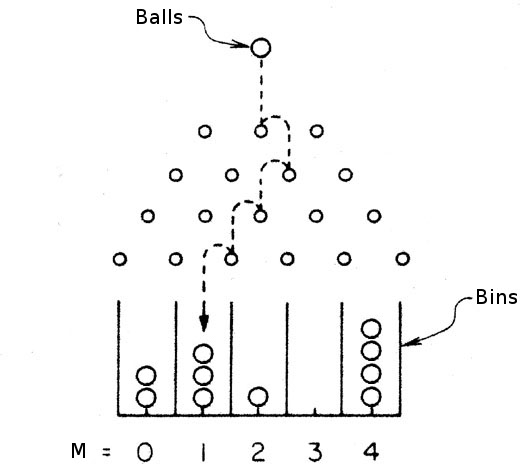
\includegraphics[width=\linewidth]{figures/BnB.jpeg}
	\caption[Caption]{Balls-and-bins problem\footnotemark}
	\label{fig:balls-and-bins}
\end{figure}
\footnotetext{Figure inspired from \autocite{bnb}}
\par
Using the balls-and-bins approach we model processes as bins and events as balls and calculate how many balls need to be \textit{thrown} such that every bin contains at least one ball with arbitrarily high probability. With this approach the number of messages transmitted per process per round is logarithmic in the number of processes, therefore the number of messages sent in the system is low and uniform over all processes. Thanks to these approaches, \epto is highly resilient with  imperfect networks and highly scalable as the network grow, while always providing total order.
\subsection{Contributions}
Until now, the creators of \epto have only tested this algorithm in a simulated environment. In this work, we implement \epto in pure Kotlin\footnote{\href{https://kotlinlang.org/}{https://kotlinlang.org/}} and introduce a benchmarking framework called \sys to show that \epto is suitable for real-world large-scale distributed systems. We compare \epto to the deterministic total order algorithm provided by \jgroups \autocite{jgroups} in both stable and unstable environments. \epto uses a PSS CYCLON \autocite{Voulgaris2005} to obtain a random view. 
Peers discover other peers through a tracker that keeps track of dead and alive peers when they first join the network.
Note that this is only used for bootstrap and is not required in the regular operation of the algorithm.
These benchmarks can easily be launched and scaled on a cluster using Docker and Docker Swarm. Furthermore, we can inject synthetic or real churn using the Failure Trace Archive databases\footnote{\href{http://fta.scem.uws.edu.au/}{http://fta.scem.uws.edu.au/}} in the system. \sys is open-sourced on Github\footnote{\href{https://github.com/jocelynthode/EpTOTester}{https://github.com/jocelynthode/EpTOTester}}. Finally we want to emphasize that few works evaluate such protocols in a really large scale \autocites[]{Chandra2007}[]{Maia2011}.
\par
The next sections present our benchmarking solution and the results obtained. Section \ref{sec:definitions} defines the terms used in the paper. Section \ref{sec:background} presents the \epto architecture and related work. Section \ref{sec:epto} presents \sys and the architecture of our implementation. Section \ref{sec:evaluation} shows and explains the results obtained as well as the limitations our project faced. We then present possible future work in Section \ref{sec:future-work}. We finally conclude in Section \ref{sec:conclusion}.
